\documentclass[8pt,aspectratio=169]{beamer}
\usetheme{Madrid}
\usepackage{graphicx}
\usepackage{booktabs}
\usepackage{adjustbox}
\usepackage{multicol}
\usepackage{amsmath}
\usepackage{amssymb}
\usepackage{tikz}
\usepackage{hyperref}
\usepackage{algorithm}
\usepackage{algorithmic}
\usepackage{colortbl}
\usepackage{pgfplots}
\pgfplotsset{compat=1.18}

% TikZ libraries for comics, diagrams, stakeholder maps
\usetikzlibrary{arrows.meta,positioning,shapes.callouts,shapes.geometric,decorations.pathreplacing}

% Color definitions
\definecolor{mlblue}{RGB}{0,102,204}
\definecolor{mlpurple}{RGB}{51,51,178}
\definecolor{mllavender}{RGB}{173,173,224}
\definecolor{mllavender2}{RGB}{193,193,232}
\definecolor{mllavender3}{RGB}{204,204,235}
\definecolor{mllavender4}{RGB}{214,214,239}
\definecolor{mlorange}{RGB}{255, 127, 14}
\definecolor{mlgreen}{RGB}{44, 160, 44}
\definecolor{mlred}{RGB}{214, 39, 40}
\definecolor{mlgray}{RGB}{127, 127, 127}
\definecolor{lightgray}{RGB}{240, 240, 240}
\definecolor{midgray}{RGB}{180, 180, 180}

% NEW COLORS for mini-lecture
\definecolor{dfteal}{RGB}{0,128,128}
\definecolor{dfred}{RGB}{180,30,30}

% Backward compatibility
\colorlet{MLPurple}{mlpurple}
\colorlet{MLBlue}{mlblue}
\colorlet{MLOrange}{mlorange}
\colorlet{MLGreen}{mlgreen}
\colorlet{MLRed}{mlred}
\colorlet{MLLavender}{mllavender}
\colorlet{MLGray}{mlgray}

% Theme colors (exact Madrid settings)
\setbeamercolor{palette primary}{bg=mllavender3,fg=mlpurple}
\setbeamercolor{palette secondary}{bg=mllavender2,fg=mlpurple}
\setbeamercolor{palette tertiary}{bg=mllavender,fg=white}
\setbeamercolor{palette quaternary}{bg=mlpurple,fg=white}
\setbeamercolor{structure}{fg=mlpurple}
\setbeamercolor{section in toc}{fg=mlpurple}
\setbeamercolor{subsection in toc}{fg=mlblue}
\setbeamercolor{title}{fg=mlpurple}
\setbeamercolor{frametitle}{fg=mlpurple,bg=mllavender3}
\setbeamercolor{block title}{bg=mllavender2,fg=mlpurple}
\setbeamercolor{block body}{bg=mllavender4,fg=black}
\setbeamertemplate{navigation symbols}{}
\setbeamertemplate{itemize items}[circle]
\setbeamertemplate{enumerate items}[default]
\setbeamersize{text margin left=5mm,text margin right=5mm}

% Footer
\setbeamertemplate{footline}{
  \leavevmode%
  \hbox{%
    \begin{beamercolorbox}[wd=.333333\paperwidth,ht=2.25ex,dp=1ex,center]{author in head/foot}%
      \usebeamerfont{author in head/foot}Methods and Algorithms
    \end{beamercolorbox}%
    \begin{beamercolorbox}[wd=.333333\paperwidth,ht=2.25ex,dp=1ex,center]{title in head/foot}%
      \usebeamerfont{title in head/foot}MSc Data Science
    \end{beamercolorbox}%
    \begin{beamercolorbox}[wd=.333333\paperwidth,ht=2.25ex,dp=1ex,right]{date in head/foot}%
      \usebeamerfont{date in head/foot}\insertframenumber{} / \inserttotalframenumber\hspace*{2ex}
    \end{beamercolorbox}}%
  \vskip0pt%
}

\newcommand{\bottomnote}[1]{%
\vfill
\vspace{-2mm}
\textcolor{mllavender2}{\rule{\textwidth}{0.4pt}}
\vspace{1mm}
\footnotesize
\textbf{#1}
}

\newenvironment{compactlist}{%
  \begin{itemize}%
    \setlength{\itemsep}{2pt}%
    \setlength{\parskip}{0pt}%
    \setlength{\parsep}{0pt}%
}{%
  \end{itemize}%
}

\newcommand{\highlight}[1]{\textcolor{mlorange}{\textbf{#1}}}
\newcommand{\mathbold}[1]{\boldsymbol{#1}}

\title[Logistic Regression Mini-Lecture]{Logistic Regression}
\subtitle{A 10-Slide Mini-Lecture}
\author{Methods and Algorithms}
\institute{MSc Data Science}
\date{}

\begin{document}

%% ================================================================
%% SLIDE 1: WHY -- TikZ Comic (Dilemma)
%% ================================================================
\begin{frame}[t]{Why Would a Credit Officer Want a Probability Instead of a Rule?}
\begin{columns}[T]
\column{0.55\textwidth}
\small
\textbf{The Dilemma}
\begin{compactlist}
\item A loan applicant scores 680 -- right at the boundary
\item The rulebook says ``approve above 700, deny below 650'' but says nothing about 680
\item A linear model predicts repayment of 1.3 -- but what does that even mean?
\end{compactlist}

\vspace{2mm}
What if instead of a number, you got the probability of default?

\begin{block}{Insight}
\scriptsize Logistic regression replaces arbitrary cutoffs with calibrated probabilities: $P(\text{default})$ maps every applicant to a number between 0 and 1.
\end{block}

\column{0.42\textwidth}
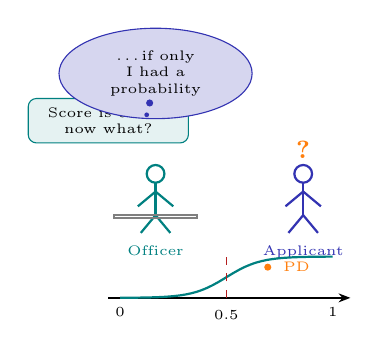
\begin{tikzpicture}[scale=0.75]
% Officer stick figure
\draw[dfteal, thick] (1,2.1) circle (0.15);
\draw[dfteal, thick] (1,1.95) -- (1,1.4);
\draw[dfteal, thick] (1,1.8) -- (0.7,1.55);
\draw[dfteal, thick] (1,1.8) -- (1.3,1.55);
\draw[dfteal, thick] (1,1.4) -- (0.75,1.1);
\draw[dfteal, thick] (1,1.4) -- (1.25,1.1);
\node[dfteal, below, font=\tiny] at (1,1.05) {Officer};
% Desk
\draw[mlgray, thick] (0.3,1.35) rectangle (1.7,1.4);
% Applicant stick figure
\draw[mlpurple, thick] (3.5,2.1) circle (0.15);
\draw[mlpurple, thick] (3.5,1.95) -- (3.5,1.4);
\draw[mlpurple, thick] (3.5,1.8) -- (3.2,1.55);
\draw[mlpurple, thick] (3.5,1.8) -- (3.8,1.55);
\draw[mlpurple, thick] (3.5,1.4) -- (3.25,1.1);
\draw[mlpurple, thick] (3.5,1.4) -- (3.75,1.1);
\node[mlpurple, below, font=\tiny] at (3.5,1.05) {Applicant};
\node[mlorange, font=\small\bfseries] at (3.5,2.5) {?};
% Speech bubble from Officer
\node[draw=dfteal, fill=dfteal!10, rounded corners=3pt,
      font=\tiny, text width=1.8cm, align=center]
      at (0.2,3.0) {Score is 680\ldots\ now what?};
% Thought bubble from Officer
\node[draw=mlpurple, fill=mllavender4, ellipse,
      font=\tiny, text width=1.5cm, align=center]
      at (1.0,3.8) {\ldots if only I had a probability};
\fill[mlpurple] (0.85,3.1) circle (0.04);
\fill[mlpurple] (0.9,3.3) circle (0.06);
% Number line 0 to 1 with sigmoid
\draw[-{Stealth[length=1.5mm]}, thick] (0.2,0) -- (4.3,0);
\node[font=\tiny, below] at (0.4,0) {0};
\node[font=\tiny, below] at (4.0,0) {1};
\node[font=\tiny, below] at (2.2,-0.05) {0.5};
% Sigmoid curve
\draw[dfteal, thick, domain=0.4:4.0, samples=40]
  plot (\x, {0.7/(1+exp(-3.5*(\x-2.2)))});
% Dashed threshold at 0.5
\draw[dfred, dashed] (2.2,0) -- (2.2,0.7);
% PD dot
\fill[mlorange] (2.9,0.52) circle (0.06);
\node[mlorange, font=\tiny, right] at (3.0,0.52) {PD};
\end{tikzpicture}
\end{columns}

\bottomnote{Logistic regression outputs $P(Y{=}1|X)$ -- a calibrated probability, not an unbounded score}
\end{frame}

%% ================================================================
%% SLIDE 2: FEEL -- Text-Only with Reflection Prompt
%% ================================================================
\begin{frame}[t]{Predicting an Outcome -- Did You Think in Probabilities?}
\begin{columns}[T]
\column{0.55\textwidth}
\small
\textbf{Think Before You Compute}

\footnotesize
Imagine you are reviewing a stack of loan applications. Without any model, you instinctively sort them: this one looks safe, that one is risky, this one could go either way. You are not assigning 0 or 1. You are assigning a feeling of likelihood -- ``probably fine'', ``probably not'', ``fifty-fifty''. That is a probability.

\begin{compactlist}
\item How confident were you in each assessment?
\item Did you use features like income, employment, or debt?
\item Were some features more important than others?
\end{compactlist}

\begin{exampleblock}{Reflection Prompt}
\scriptsize Write down one real decision you made this week where you mentally estimated a probability. What features did you use?
\end{exampleblock}

\column{0.42\textwidth}
\footnotesize
\vspace{4mm}
\fcolorbox{mlpurple}{mllavender4}{\parbox{0.85\columnwidth}{%
\textbf{Pause and reflect:}

\vspace{2mm}
When you last decided whether to bring an umbrella, you estimated $P(\text{rain})$ from features: clouds, forecast, season. You did not predict rain $= 1.3$.

\vspace{2mm}
\textbf{That is logistic regression.}
}}
\end{columns}

\bottomnote{Human intuition naturally produces probabilities -- logistic regression formalizes this into a trainable model}
\end{frame}

%% ================================================================
%% SLIDE 3: WHAT -- Comparison Table
%% ================================================================
\begin{frame}[t]{What Makes Logistic Regression Different from Linear Regression and Decision Trees?}
\begin{columns}[T]
\column{0.55\textwidth}
\small
\textbf{Taxonomy of Classifiers}

\vspace{1mm}
\footnotesize
\begin{tabular}{@{}l c c c@{}}
\toprule
\textbf{Property} & \textbf{\textcolor{dfteal}{LogReg}} & \textbf{LinReg} & \textbf{Dec.\ Tree} \\
\midrule
\rowcolor{mllavender4}
Output & Prob.\ & Real & Class/Prob.\ \\
Boundary & Linear & N/A & Axis-aligned \\
\rowcolor{mllavender4}
Loss & Cross-ent.\ & MSE & Gini/Entropy \\
Interpret.\ & High (OR) & High & Medium \\
\rowcolor{mllavender4}
Regularize & L1/L2/EN & L1/L2 & Pruning \\
Calibration & Native & Poor & Poor \\
\bottomrule
\end{tabular}

\vspace{2mm}
\scriptsize\textbf{Logistic regression is the only method here that directly outputs well-calibrated probabilities.}

\begin{block}{Insight}
\scriptsize LogReg occupies a unique niche: parametric, interpretable, probabilistic, and naturally calibrated -- which is why regulators love it.
\end{block}

\column{0.42\textwidth}
\footnotesize
\vspace{2mm}
\colorbox{dfteal!15}{\parbox{0.9\columnwidth}{\textbf{LogReg:} Probabilistic, parametric, linear boundary}}

\vspace{3mm}
\colorbox{mlorange!15}{\parbox{0.9\columnwidth}{\textbf{LinReg:} Continuous output, no classification}}

\vspace{3mm}
\colorbox{mlpurple!15}{\parbox{0.9\columnwidth}{\textbf{Tree:} Non-parametric, axis-aligned, uncalibrated}}
\end{columns}

\bottomnote{Odds ratio interpretation: each coefficient tells you the multiplicative change in odds per unit feature change}
\end{frame}

%% ================================================================
%% SLIDE 4: CASE -- Step Diagram (TikZ Flow)
%% ================================================================
\begin{frame}[t]{How Does One Loan Application Travel from Features to Probability?}
\begin{columns}[T]
\column{0.55\textwidth}
\small
\textbf{One Prediction, Step by Step}
\begin{compactlist}
\item Applicant arrives with features: income=50k, debt-ratio=0.35, employment=4yr
\item Compute linear combination: $z = w_0 + w_1 \cdot \text{income} + w_2 \cdot \text{debt} + w_3 \cdot \text{empl.}$
\item Apply sigmoid: $P(\text{default}) = \frac{1}{1 + e^{-z}}$
\item Compare to threshold (e.g., 0.5): if $P > 0.5$, predict default
\item Bank uses the raw probability for capital reserves (Basel PD)
\end{compactlist}

\begin{block}{Insight}
\scriptsize The sigmoid is the bridge: it maps any real number $z$ to a probability in $(0,1)$. The threshold is a business decision, not a model decision.
\end{block}

\column{0.42\textwidth}
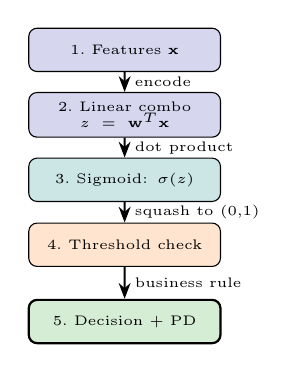
\begin{tikzpicture}[scale=0.75,
  stepnode/.style={draw, rounded corners=3pt, font=\tiny,
    text width=2.2cm, align=center, minimum height=0.55cm},
  arr/.style={-{Stealth[length=2mm]}, thick}]
% Nodes
\node[stepnode, fill=mllavender4] (s1) at (1.5,5.0) {1.\ Features $\mathbf{x}$};
\node[stepnode, fill=mllavender4] (s2) at (1.5,3.9) {2.\ Linear combo $z = \mathbf{w}^T\mathbf{x}$};
\node[stepnode, fill=dfteal!20]   (s3) at (1.5,2.8) {3.\ Sigmoid: $\sigma(z)$};
\node[stepnode, fill=mlorange!20] (s4) at (1.5,1.7) {4.\ Threshold check};
\node[stepnode, fill=mlgreen!20, thick] (s5) at (1.5,0.4) {5.\ Decision + PD};
% Arrows with labels
\draw[arr] (s1) -- (s2) node[midway, right, font=\tiny] {encode};
\draw[arr] (s2) -- (s3) node[midway, right, font=\tiny] {dot product};
\draw[arr] (s3) -- (s4) node[midway, right, font=\tiny] {squash to (0,1)};
\draw[arr] (s4) -- (s5) node[midway, right, font=\tiny] {business rule};
\end{tikzpicture}
\end{columns}

\bottomnote{The model outputs $P(\text{default})$; the threshold is chosen by the business based on cost trade-offs}
\end{frame}

%% ================================================================
%% SLIDE 5: HOW -- Side-by-Side Architecture
%% ================================================================
\begin{frame}[t]{Who Should Fit the Model -- Gradient Descent, Newton, or a Library?}
\begin{columns}[T]
\column{0.55\textwidth}
\small
\textbf{Three Optimization Approaches}
\begin{compactlist}
\item \textbf{Gradient Descent}: update $\mathbf{w} = \mathbf{w} - \eta \frac{X^T(\mathbf{p}-\mathbf{y})}{n}$, simple but slow
\item \textbf{Newton-Raphson (IRLS)}: uses Hessian, converges quadratically, standard in statsmodels/R
\item \textbf{L-BFGS}: quasi-Newton, memory-efficient, default in scikit-learn
\end{compactlist}

\vspace{1mm}
\scriptsize All three minimize the same convex cross-entropy loss -- global optimum guaranteed.

\begin{block}{Insight}
\scriptsize Cross-entropy is convex in the weights, so every optimizer converges to the same solution. The choice is about speed, not correctness.
\end{block}

\column{0.42\textwidth}
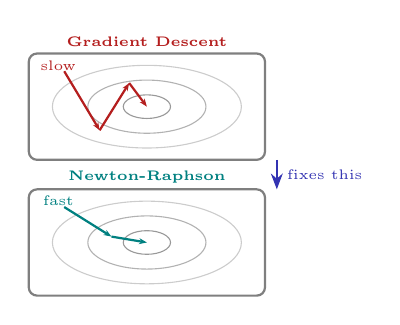
\begin{tikzpicture}[scale=0.75]
% --- Top box: Gradient Descent (slow) ---
\node[font=\tiny\bfseries, dfred] at (2.2,4.6) {Gradient Descent};
\draw[mlgray, thick, rounded corners=3pt] (0.2,2.6) rectangle (4.2,4.4);
% Contour ellipses
\draw[mlgray!40] (2.2,3.5) ellipse (1.6 and 0.7);
\draw[mlgray!60] (2.2,3.5) ellipse (1.0 and 0.45);
\draw[mlgray!80] (2.2,3.5) ellipse (0.4 and 0.2);
% Zigzag arrows (slow)
\draw[-{Stealth[length=1mm]}, dfred, thick]
  (0.8,4.1) -- (1.4,3.1);
\draw[-{Stealth[length=1mm]}, dfred, thick]
  (1.4,3.1) -- (1.9,3.9);
\draw[-{Stealth[length=1mm]}, dfred, thick]
  (1.9,3.9) -- (2.2,3.5);
\node[font=\tiny, dfred] at (0.7,4.2) {slow};
% --- Bottom box: Newton-Raphson (fast) ---
\node[font=\tiny\bfseries, dfteal] at (2.2,2.3) {Newton-Raphson};
\draw[mlgray, thick, rounded corners=3pt] (0.2,0.3) rectangle (4.2,2.1);
% Contour ellipses
\draw[mlgray!40] (2.2,1.2) ellipse (1.6 and 0.7);
\draw[mlgray!60] (2.2,1.2) ellipse (1.0 and 0.45);
\draw[mlgray!80] (2.2,1.2) ellipse (0.4 and 0.2);
% Direct arrows (fast)
\draw[-{Stealth[length=1mm]}, dfteal, thick]
  (0.8,1.8) -- (1.6,1.3);
\draw[-{Stealth[length=1mm]}, dfteal, thick]
  (1.6,1.3) -- (2.2,1.2);
\node[font=\tiny, dfteal] at (0.7,1.9) {fast};
% Arrow between boxes
\draw[-{Stealth[length=2mm]}, mlpurple, thick]
  (4.4,2.6) -- (4.4,2.1) node[midway, right, font=\tiny] {fixes this};
\end{tikzpicture}
\end{columns}

\bottomnote{Newton-Raphson converges in 5--10 iterations vs.\ hundreds for gradient descent -- but requires Hessian inversion}
\end{frame}

%% ================================================================
%% SLIDE 6: RISK -- TikZ Comic (Failure Scene)
%% ================================================================
\begin{frame}[t]{What Could Go Wrong If You Trust the Default Threshold?}
\begin{columns}[T]
\column{0.55\textwidth}
\small
\textbf{Three Ways Logistic Regression Fails Silently}
\begin{compactlist}
\item \textbf{Class imbalance}: 99\% non-default means predicting ``no default'' always gets 99\% accuracy
\item \textbf{Separation}: if one feature perfectly predicts the outcome, coefficients explode to infinity
\item \textbf{Non-linear boundaries}: logistic regression draws a straight line -- curved patterns get misclassified
\end{compactlist}

\begin{block}{Insight}
\scriptsize The default 0.5 threshold is almost never optimal in finance. Fraud detection might use 0.1; credit scoring might use 0.3.
\end{block}

\column{0.42\textwidth}
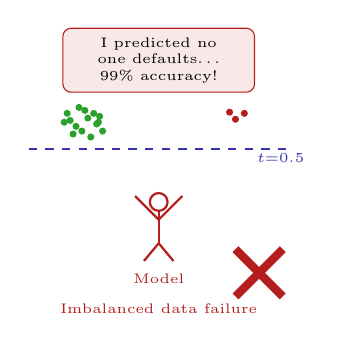
\begin{tikzpicture}[scale=0.75]
% Model stick figure in center (distress)
\draw[dfred, thick] (2.5,2.1) circle (0.15);
\draw[dfred, thick] (2.5,1.95) -- (2.5,1.4);
% Arms raised in distress
\draw[dfred, thick] (2.5,1.8) -- (2.1,2.2);
\draw[dfred, thick] (2.5,1.8) -- (2.9,2.2);
\draw[dfred, thick] (2.5,1.4) -- (2.25,1.1);
\draw[dfred, thick] (2.5,1.4) -- (2.75,1.1);
\node[dfred, below, font=\tiny] at (2.5,1.05) {Model};
% Imbalanced data dots -- large green cluster (non-default)
\foreach \dx/\dy in {0/0, 0.25/0.12, -0.2/0.18, 0.15/-0.1,
  -0.1/0.08, 0.3/0.25, -0.25/0.3, 0.05/0.35,
  0.35/0.0, -0.3/0.15, 0.2/0.3, -0.15/-0.05,
  0.1/0.22, -0.05/0.4, 0.28/0.15} {
  \fill[mlgreen] (1.2+\dx, 3.3+\dy) circle (0.06);
}
% Tiny red cluster (default)
\foreach \dx/\dy in {0/0, 0.15/0.1, -0.1/0.12} {
  \fill[dfred] (3.8+\dx, 3.5+\dy) circle (0.06);
}
% Dashed threshold line
\draw[mlpurple, dashed, thick] (0.3,3.0) -- (4.7,3.0);
\node[font=\tiny, mlpurple, right] at (4.0,2.85) {$t{=}0.5$};
% Speech bubble
\node[draw=dfred, fill=dfred!10, rounded corners=3pt,
      font=\tiny, text width=2.2cm, align=center]
      at (2.5,4.5) {I predicted no one defaults\ldots\ 99\% accuracy!};
% Large red X
\draw[dfred, line width=3pt] (3.8,0.5) -- (4.6,1.3);
\draw[dfred, line width=3pt] (3.8,1.3) -- (4.6,0.5);
% Label
\node[font=\tiny, dfred] at (2.5,0.3) {Imbalanced data failure};
\end{tikzpicture}
\end{columns}

\bottomnote{Always evaluate with AUC, precision-recall, and Gini -- never with accuracy alone on imbalanced data}
\end{frame}

%% ================================================================
%% SLIDE 7: WHERE -- External Chart (PDF)
%% ================================================================
\begin{frame}[t]{Why Does Every Credit Risk Team Start with Logistic Regression?}
\begin{columns}[T]
\column{0.55\textwidth}
\small
\textbf{Logistic Regression as the Regulatory Baseline}
\begin{compactlist}
\item Interpretable: every coefficient has a direct odds-ratio interpretation
\item Auditable: regulators can inspect and validate each feature's contribution
\item Calibrated: output probabilities match observed default rates
\item Stable: small data changes produce small coefficient changes
\end{compactlist}

\vspace{1mm}
\scriptsize The ROC curve shows how well the model discriminates defaulters from non-defaulters at every threshold.

\begin{block}{Insight}
\scriptsize Logistic regression is not popular in credit scoring because it is the best predictor -- it is popular because it is the most interpretable predictor.
\end{block}

\column{0.42\textwidth}
\vspace{2mm}
\includegraphics[width=\textwidth]{04_roc_curve/chart.pdf}
\end{columns}

\bottomnote{Gini $= 2 \cdot \text{AUC} - 1$: industry standard. Gini $> 0.40$ acceptable; Gini $> 0.60$ good for credit scoring}
\end{frame}

%% ================================================================
%% SLIDE 8: IMPACT -- Stakeholder Map
%% ================================================================
\begin{frame}[t]{Who Wins and Who Loses When a Bank Switches to Logistic Regression?}
\begin{columns}[T]
\column{0.55\textwidth}
\small
\textbf{Stakeholder Analysis}
\begin{compactlist}
\item \textbf{Winners}: Risk managers (calibrated PD), regulators (interpretable model), applicants (consistent decisions), capital planning (accurate reserves)
\item \textbf{Losers}: Data scientists wanting complex models, branch managers (discretion reduced), anyone with non-linear intuition
\end{compactlist}

\vspace{1mm}
\scriptsize LogReg shifts power from subjective judgment to auditable probability.

\begin{block}{Insight}
\scriptsize In regulated finance, interpretability is not optional -- it is a legal requirement under Basel II/III and GDPR Article 22.
\end{block}

\column{0.42\textwidth}
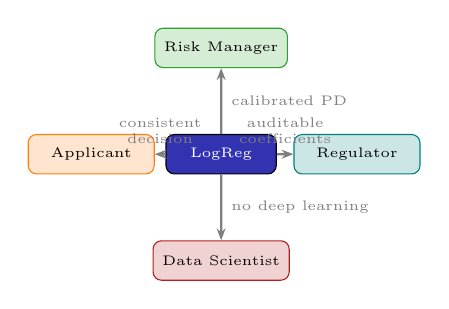
\begin{tikzpicture}[scale=0.75,
  actor/.style={draw, rounded corners=3pt, font=\tiny,
    minimum width=1.6cm, minimum height=0.5cm, align=center},
  arr/.style={-{Stealth[length=1.5mm]}, thick, mlgray}]
% Center
\node[actor, fill=mlpurple, text=white, minimum width=1.4cm] (lr) at (2.2,2.2) {LogReg};
% Top: Risk Manager
\node[actor, fill=mlgreen!20, draw=mlgreen] (risk) at (2.2,4.0) {Risk Manager};
\draw[arr] (lr) -- (risk) node[midway, right, font=\tiny] {calibrated PD};
% Right: Regulator
\node[actor, fill=dfteal!20, draw=dfteal] (reg) at (4.5,2.2) {Regulator};
\draw[arr] (lr) -- (reg) node[midway, above, font=\tiny, text width=1.2cm, align=center] {auditable coefficients};
% Bottom: Data Scientist
\node[actor, fill=dfred!20, draw=dfred] (ds) at (2.2,0.4) {Data Scientist};
\draw[arr] (lr) -- (ds) node[midway, right, font=\tiny] {no deep learning};
% Left: Applicant
\node[actor, fill=mlorange!20, draw=mlorange] (app) at (0,2.2) {Applicant};
\draw[arr] (lr) -- (app) node[midway, above, font=\tiny, text width=1.2cm, align=center] {consistent decision};
\end{tikzpicture}
\end{columns}

\bottomnote{Basel IRB requires banks to demonstrate PD model validity annually -- logistic regression passes this test}
\end{frame}

%% ================================================================
%% SLIDE 9: SO WHAT -- Balance Scale
%% ================================================================
\begin{frame}[t]{3 Questions That Reveal Whether Logistic Regression Is the Right Model}
\begin{columns}[T]
\column{0.55\textwidth}
\small
\textbf{The Decision Framework}
\begin{enumerate}
\setlength{\itemsep}{2pt}
\item \textbf{Is the outcome binary (or ordinal)?} -- If continuous, use linear regression; if multi-class, consider softmax
\item \textbf{Is interpretability required?} -- If regulators demand coefficient explanations, LogReg wins
\item \textbf{Is the decision boundary approximately linear?} -- If strongly non-linear, consider tree ensembles or feature engineering
\end{enumerate}

\vspace{1mm}
\scriptsize If all three answers are yes, logistic regression is the right first model.

\begin{block}{Insight}
\scriptsize Logistic regression should be your first model for any binary classification problem in a regulated environment.
\end{block}

\column{0.42\textwidth}
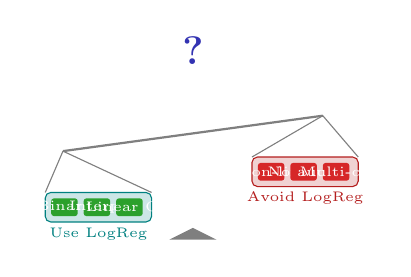
\begin{tikzpicture}[scale=0.75]
% Fulcrum
\fill[mlgray] (2.5,0.2) -- (2.1,0) -- (2.9,0) -- cycle;
% Beam (tilted: left lower = Use LogReg wins)
\draw[thick, mlgray] (0.3,1.5) -- (4.7,2.1);
% Left pan: Use LogReg
\draw[mlgray] (0.3,1.5) -- (0.0,0.8);
\draw[mlgray] (0.3,1.5) -- (1.8,0.8);
\draw[dfteal, fill=dfteal!20, rounded corners=2pt]
  (0.0,0.3) rectangle (1.8,0.8);
\foreach \i/\txt in {0/Binary, 1/Interp., 2/Linear OK} {
  \fill[mlgreen, rounded corners=1pt]
    (0.1+\i*0.55, 0.4) rectangle (0.55+\i*0.55, 0.7);
  \node[font=\tiny, white] at (0.33+\i*0.55, 0.55) {\txt};
}
\node[font=\tiny, dfteal] at (0.9,0.1) {Use LogReg};
% Right pan: Avoid LogReg
\draw[mlgray] (4.7,2.1) -- (3.5,1.4);
\draw[mlgray] (4.7,2.1) -- (5.3,1.4);
\draw[dfred, fill=dfred!20, rounded corners=2pt]
  (3.5,0.9) rectangle (5.3,1.4);
\foreach \i/\txt in {0/Non-lin., 1/No audit, 2/Multi-cls} {
  \fill[mlred, rounded corners=1pt]
    (3.6+\i*0.55, 1.0) rectangle (4.05+\i*0.55, 1.3);
  \node[font=\tiny, white] at (3.83+\i*0.55, 1.15) {\txt};
}
\node[font=\tiny, dfred] at (4.4,0.7) {Avoid LogReg};
% Question mark
\node[mlpurple, font=\Large\bfseries] at (2.5,3.2) {?};
\end{tikzpicture}
\end{columns}

\bottomnote{Even when you suspect non-linearity, start with LogReg as a baseline -- you need something to beat}
\end{frame}

%% ================================================================
%% SLIDE 10: ACT -- Activity Frame
%% ================================================================
\begin{frame}[t]{Can You Evaluate This Real Credit Scoring Problem?}
\begin{columns}[T]
\column{0.55\textwidth}
\small
\textbf{The Scenario}

\footnotesize
A consumer bank wants to predict credit card default. Features: monthly income, credit utilization ratio, number of late payments (past 12 months), years with current employer, total debt. Dataset has 10,000 accounts with 3\% default rate.

\begin{compactlist}
\item Apply the 3-question framework from the previous slide
\item Decide: Is logistic regression appropriate here?
\item If yes: what threshold would you choose (hint: 3\% default rate)?
\item What single metric would you report to the regulator?
\end{compactlist}

\begin{exampleblock}{Deliverable}
\scriptsize Fill in the table. Be prepared to defend your verdict to a skeptical Basel auditor.
\end{exampleblock}

\column{0.42\textwidth}
\footnotesize
\vspace{2mm}
\begin{tabular}{@{}l p{2.8cm}@{}}
\toprule
\textbf{Question} & \textbf{Your Answer} \\
\midrule
Binary outcome? & \rule{2.5cm}{0.4pt} \\[3pt]
Interpretable needed? & \rule{2.5cm}{0.4pt} \\[3pt]
Linear boundary OK? & \rule{2.5cm}{0.4pt} \\[3pt]
\textbf{Verdict} & \rule{2.5cm}{0.4pt} \\[3pt]
Recommended threshold & \rule{2.5cm}{0.4pt} \\[3pt]
Key metric for regulator & \rule{2.5cm}{0.4pt} \\
\bottomrule
\end{tabular}
\end{columns}

\bottomnote{Hint: with 3\% default rate, accuracy is meaningless. Think about Gini, AUC, or precision-recall.}
\end{frame}

\end{document}
